% ------------------------------------------------------------------------------
% TYPO3 Version 9.1 - What's New - Chapter "Backend User Interface" (English Version)
%
% @author	Michael Schams <schams.net>
% @license	Creative Commons BY-NC-SA 3.0
% @link		http://typo3.org/download/release-notes/whats-new/
% @language	English
% ------------------------------------------------------------------------------
% LTXE-CHAPTER-UID:		07b25346-95b1df21-a6ebe09a-49f53f41
% LTXE-CHAPTER-NAME:	Backend User Interface
% ------------------------------------------------------------------------------

\section{Backend User Interface}
\begin{frame}[fragile]
	\frametitle{Backend User Interface}

	\begin{center}\huge{Chapter 1:}\end{center}
	\begin{center}\huge{\color{typo3darkgrey}\textbf{Backend User Interface}}\end{center}

\end{frame}

% ------------------------------------------------------------------------------
% LTXE-SLIDE-START
% LTXE-SLIDE-UID:		e0ad33fe-9f5b1a93-218b12e9-6410e8f5
% LTXE-SLIDE-TITLE:		Added New Main Module Site Management
% LTXE-SLIDE-REFERENCE:	Feature-83637-AddedNewMainModuleSiteManagement.rst
% ------------------------------------------------------------------------------

\begin{frame}[fragile]
	\frametitle{Backend User Interface}
	\framesubtitle{Site Management}

	A new main module \textbf{Site Management} has been introduced to the TYPO3 core.
	Its main purpose is to host functions related to the configuration of the site,
	e.g. languages, domains and routing.

	\begin{columns}[T]
		\begin{column}{.4\textwidth}
			\begin{figure}\vspace*{-0.4cm}
				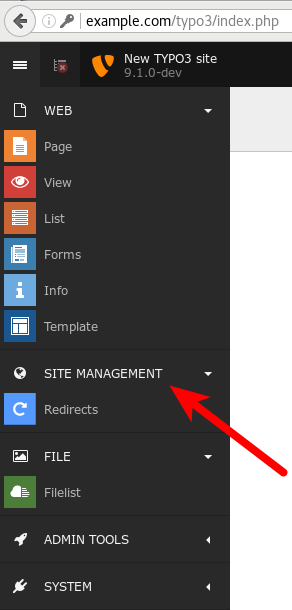
\includegraphics[width=0.45\linewidth]{BackendUserInterface/AddedNewMainModuleSiteManagement.png}
			\end{figure}
		\end{column}
		\begin{column}{.5\textwidth}
			The new system extension \texttt{EXT:redirects} builds the first component
			of this main module (see next page for details).
		\end{column}
		\begin{column}{.1\textwidth}
		\end{column}
	\end{columns}

\end{frame}

% ------------------------------------------------------------------------------
% LTXE-SLIDE-START
% LTXE-SLIDE-UID:		8bd6b85d-ed8c77e3-94a40b39-e15bb504
% LTXE-SLIDE-TITLE:		System Extension "Redirects" Has Been Added
% LTXE-SLIDE-REFERENCE:	Feature-83631-SystemExtensionRedirectsHasBeenAdded.rst
% ------------------------------------------------------------------------------

\begin{frame}[fragile]
	\frametitle{Backend User Interface}
	\framesubtitle{Redirects}

	New module allows integrators and editors to configure redirects.
	The function contains a simple hit counter (needs to be enabled) and
	redirects can be set up unlimited or for a specific time period.

	\begin{figure}
		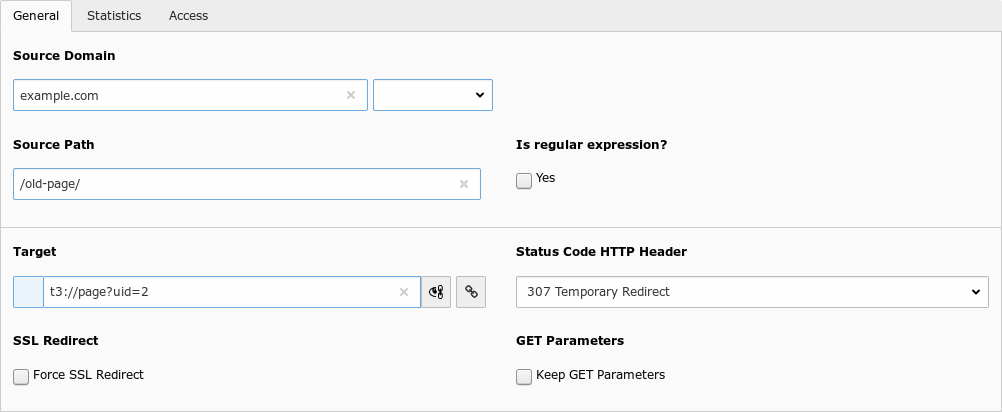
\includegraphics[width=0.8\linewidth]{BackendUserInterface/SystemExtensionRedirectsHasBeenAdded.png}
	\end{figure}

\end{frame}

% ------------------------------------------------------------------------------
% LTXE-SLIDE-START
% LTXE-SLIDE-UID:		e10a0f89-e91ecdb3-928841b6-1a84fc50
% LTXE-SLIDE-TITLE:		Show Fieldname Next To Title In Debug Mode
% LTXE-SLIDE-REFERENCE:	Feature-83461-ShowFieldnameNextToTitleInDebugMode.rst
% ------------------------------------------------------------------------------

\begin{frame}[fragile]
	\frametitle{Backend User Interface}
	\framesubtitle{Field Names in Debug Mode}

	\begin{itemize}

		\item TYPO3 integrators and developers often deal with input fields in the backend,
			e.g. when setting up access permissions or during TsConfig configuration.

		\item Instead of looking into the source code of the browser, field names are shown
			for each field generated by the FormEngine now.

		\item This applies to users with administrator privileges only and requires that
			the debug mode is enabled in TYPO3:

			\smaller
				\texttt{\$GLOBALS['TYPO3\_CONF\_VARS']['BE']['debug']}
			\normalsize

	\end{itemize}

	\begin{figure}
		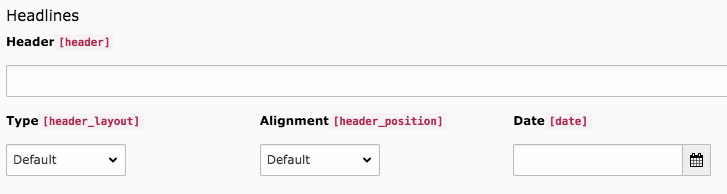
\includegraphics[width=0.60\linewidth]{BackendUserInterface/ShowFieldnameNextToTitleInDebugMode.png}
	\end{figure}

\end{frame}

% ------------------------------------------------------------------------------
